% This file was created by tikzplotlib v0.9.2.
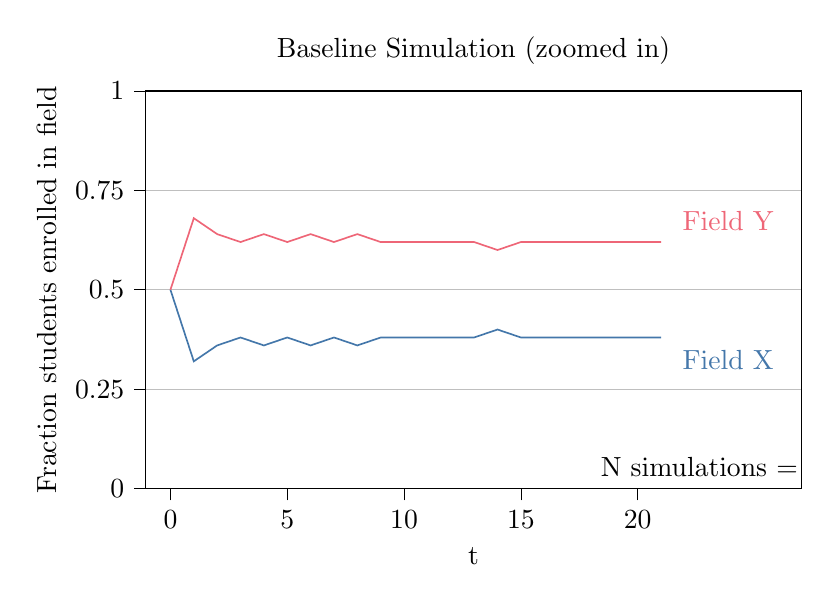
\begin{tikzpicture}

\definecolor{color0}{rgb}{0.266666666666667,0.466666666666667,0.666666666666667}
\definecolor{color1}{rgb}{0.933333333333333,0.4,0.466666666666667}

\begin{axis}[
height=6.6314113761540705cm,
tick align=outside,
tick pos=left,
title={Baseline Simulation (zoomed in)},
width=9.904475999999999cm,
x grid style={white!69.0196078431373!black},
xlabel={t},
xmin=-1.05, xmax=27,
xtick style={color=black},
xtick={0,5,10,15,20},
xticklabels={\(\displaystyle 0\),\(\displaystyle 5\),\(\displaystyle 10\),\(\displaystyle 15\),\(\displaystyle 20\)},
ylabel={Fraction students enrolled in field},
ymajorgrids,
ymin=0, ymax=1,
ytick style={color=black},
ytick={0,0.25,0.5,0.75,1},
yticklabels={\(\displaystyle 0\),\(\displaystyle 0.25\),\(\displaystyle 0.5\),\(\displaystyle 0.75\),\(\displaystyle 1\)}
]
\addplot [semithick, color0]
table {%
0 0.5
1 0.319999933242798
2 0.360000014305115
3 0.379999995231628
4 0.360000014305115
5 0.379999995231628
6 0.360000014305115
7 0.379999995231628
8 0.360000014305115
9 0.379999995231628
13 0.379999995231628
14 0.399999976158142
15 0.379999995231628
21 0.379999995231628
};
\addplot [semithick, color1]
table {%
0 0.5
1 0.680000066757202
2 0.639999985694885
3 0.620000004768372
4 0.639999985694885
5 0.620000004768372
6 0.639999985694885
7 0.620000004768372
8 0.639999985694885
9 0.620000004768372
13 0.620000004768372
14 0.600000023841858
15 0.620000004768372
21 0.620000004768372
};
\draw (axis cs:21.5,0.3) node[
  anchor=base west,
  text=color0,
  rotate=0.0
]{Field X};
\draw (axis cs:21.5,0.65) node[
  anchor=base west,
  text=color1,
  rotate=0.0
]{Field Y};
\draw (axis cs:18,0.03) node[
  anchor=base west,
  text=black,
  rotate=0.0
]{N simulations = 50};
\end{axis}

\end{tikzpicture}
